%!TEX root = dissertation.tex
\chapter{Taylor moment expansion filtering and smoothing}
\label{chap:tme}
This chapter is concerned with Publication~\cp{paperTME}. More specifically, this chapter presents the Taylor moment expansion (TME) scheme for approximating the statistical properties of SDE solutions, such as their mean and covariance. Based on this, we thereupon present TME-based Gaussian filters and smoothers and analyse their stability.

The chapter starts with a general discussion on the motivation and background of the TME method. In Section~\ref{sec:generator}, we briefly review diffusion processes and related infinitesimal generators which are the key ingredients of TME. Then, in Sections~\ref{sec:tme} we formally introduce TME, and in Section~\ref{sec:tme-pd} we analyse the positive definiteness of their covariance approximants. Section~\ref{sec:tme-examples} features several examples that illustrate how to use TME in practice. Finally, in Section~\ref{sec:tme-filter-smoother}, we present Gaussian approximated density filters and smoothers that leverage the TME method for approximating the predictive means and covariances of the system.

\section{Motivation}
\label{sec:tme-motivation}
Let $X(t)$ be an It\^{o} process that satisfies the SDE given by Equation~\eqref{equ:SDE}. In stochastic filtering and smoothing~\citep{Jazwinski1970, Bain2009, Sarkka2013}, it is often of interest to compute the conditional expectation of a given target function $\phi$ for any two time points $t\geq s \in\T$.  For instance, as shown in Algorithm~\ref{alg:gfs}, Gaussian approximated density filters and smoothers require to be able to compute the predictive mean and covariance of SDE solutions. These conditional expectations take the form
%
\begin{equation}
	\expec{\phi(X(t)) \cond X(s)},
	\label{equ:tme-motivation-moment}
\end{equation}
where different target functions result in different statistical quantities, such as mean, covariance or higher-order moments.

There exist several approaches to computing the expectation in Equation~\eqref{equ:tme-motivation-moment} numerically. One approach is based on forming an ODE that governs the conditional expectation in Equation~\eqref{equ:tme-motivation-moment}~\citep[see, e.g., ][]{DongbinXiu2010, Khasminskii2012, Sarkka2019}. For example, let $\phi(x) = x$, then by It\^{o}'s formula we can obtain an ODE
%
\begin{equation}
	\frac{\diff \expec{X(t) \cond X(s)}}{\diff t} = \expec{a(X(t), t)  \cond X(s) }
	\label{equ:mean-ode}
\end{equation}
%
starting from $s\in \T$. However, it is usually hard to solve the ODE in Equation~\eqref{equ:mean-ode} analytically. This is due to the fact that computing its driving term $\expec{a(X(t), t)  \cond X(s)}$ requires computing an expectation with respect to the SDE distribution, which is in general intractable analytically. One solution to this problem is to approximate the expectation using quadrature integration methods~\citep{Sarkka2007, Sarkka2010CD, Kulikova2014}, but the approximation error can accumulate in time, resulting in unstable estimation. Another solution is to iteratively form ODEs that characterise their parent driving terms. Explicitly, one can choose $\phi=a$ in the above, so as to characterise $\expec{a(X(t), t) \cond X(s)}$ by another ODE driven by some function $a'$, then choose $\phi=a'$, and so on. However, this leads to a so-called closure problem as explained in~\citet[][Section 4.4.2]{DongbinXiu2010}.

It is also common to approximate Equation~\eqref{equ:tme-motivation-moment} using numerical discretisation methods, such as Euler--Maruyama, Milstein's method, or higher-order It\^{o}--Taylor expansions~\citep{Kloeden1992}. The upside of these methods is that if the function $\phi$ happens to be a polynomial function, then these methods can give analytical approximations of Equation~\eqref{equ:tme-motivation-moment}. As an example, let $\phi(x) = (x - \expec{X(t)})\, (x - \expec{X(t)})^\trans.$ Then the Euler--Maruyama method gives the approximation
%
\begin{equation}
	\expec{\phi(X(t)) \cond X(s)} = \cov{X(t) \cond X(s)} \approx (t-s) \, b(X(s), s) \, b(X(s), s)^\trans \nonumber.
\end{equation}
%
However, for more general non-linear $\phi$ these approaches usually fail to give analytical approximations (see, e.g., Example~\ref{example-tme-benes}), and one often needs to use Monte Carlo methods to approximate the expectation. 

In the remainder of this section, we present the so-called Taylor moment expansion~\citep{Zmirou1986, Zmirou1989, Kessler1997, ZhaoTME2020} approach for computing expectations of the form given in Equation~\eqref{equ:tme-motivation-moment}. This method relies on approximating the expectation in Equation~\eqref{equ:tme-motivation-moment} in terms of a Taylor expansion up to a given order $M$ that depends on the regularity of the coefficients of the SDE verified by $X$. The terms in this expansion are expressed as iterative applications of the infinitesimal generator of the SDE at hand on the target function $\phi$ (see, Section~\ref{sec:generator} for a formal definition). When the coefficients are infinitely smooth, this method offers asymptotically exact representations. We start by giving an overview of diffusion processes and the infinitesimal generator which is an essential part of the TME method.

\section{Infinitesimal generator}
\label{sec:generator}
Diffusion processes~\citep{Dynkin1965, Ikeda1992, Ito2004} are an important subclass of continuous-time Markov processes whose transition probability densities verify certain (infinitesimal) regularities~\citep[see, e.g.,][Definition 10.8.3]{Kuo2006Book}. These processes are entirely characterised by their infinitesimal generators which are defined as follows. Let $X\colon \T \to \R^d$ be a diffusion process starting from any $x\in\R^d$ at $t_0$ and let $\phi$ be a suitable function. The operator $\A$ defined by
%
\begin{equation}
	\A \phi(x) = \lim_{t\downarrow t_0} \frac{\expec{\phi (X(t)) \cond x} - \phi (x)}{t-t_0}
	\label{equ:generator-general}
\end{equation}
%
is called the \emph{infinitesimal generator} of the diffusion $X$. Heuristically, the infinitesimal generator represents the expected rate of change of $\phi(X(t))$ around $x$. 

There are many approaches to construct diffusion processes (with desired drift and diffusion coefficients), such as the semigroup approach, the PDE approach (i.e., Kolmogorov backward equation), and the (It\^{o}'s) SDE approach~\citep{Kuo2006Book, ReneBrownianBook2012}. In particular, if one considers diffusion processes that are solutions of SDE, then their infinitesimal generators can be expressed in terms of their SDE coefficients. 

\begin{theorem}[Infinitesimal generator in It\^{o}'s SDE representation]
    \label{thm:generator-in-sde}
	Let $X \colon \T \to \R^d$ be a diffusion process that is the solution of the following time-homogeneous SDE
	\begin{equation}
		\diff X(t) = a(X(t)) \diff t + b(X(t)) \diff W(t), 
		\label{equ:t-homo-sde}
	\end{equation}
	where $a \colon \R^d \to \R^d$, $b \colon \R^d \to\R^{d\times w}$, and $W \colon \T \to \R^w$ is a Wiener process. Also let us define $\Gamma(x) \coloneqq b(x) \, b(x)^\trans$. Then, the infinitesimal generator $\A$ defined in Equation~\eqref{equ:generator-general} is given by
	\begin{equation}
		\begin{split}
			\A \phi(x) &= \sum^d_{i=1} a_{i}(x) \, \tash{\phi}{x_i}(x) + \frac{1}{2} \sum_{i,j=1}^d \Gamma_{ij}(x) \, \frac{\partial^2 \phi}{\partial x_i \, \partial x_j}(x)\\
			&\coloneqq (\nabla_x \phi(x))^\trans \, a(x) + \frac{1}{2} \tracebig{\Gamma(x) \, \hessian_x \phi(x)}
			\label{equ:generator-ito}
		\end{split}
	\end{equation}
	for any suitable $\phi\in \mathcal{C}^2(\R^d;\R)$.
	The drift and diffusion coefficients of the diffusion $X$ are then given by $a$ and $\Gamma$, respectively.
\end{theorem}
\begin{proof}
	The proof can be found, for example, in \citet[][Theorem~7.3.3]{Oksendal2003} or \citet[][Theorem 10.9.11]{Kuo2006Book}.
\end{proof}

Theorem~\ref{thm:generator-in-sde} can be extended to the case of time-dependent $x, t \mapsto \phi(x, t)$ and SDE coefficients $x, t \mapsto a(x, t)$, $x, t \mapsto b(x, t)$. For details of this, see, for example,  \citet[][Definition 5.3]{Sarkka2019}.

\section{Taylor moment expansion (TME)}
\label{sec:tme}
Recall that the aim of this section is to compute expectations of the form
\begin{equation}
	\expec{\phi(X(t)) \cond X(s)}
	\label{equ:tme-of-interests}
\end{equation}
for $t\geq s \in \T$ and any given target function $\phi$. 

The idea of TME~\citep{Zmirou1989} is to approximate Equation~\eqref{equ:tme-of-interests} by means of a Taylor expansion
%
\begin{equation}
	\expec{\phi(X(t)) \cond X(s)} \approx \sum^M_{r=0} \frac{1}{r!} \, \frac{\diff^r \expec{\phi(X(t)) \cond X(s)}}{\diff t^r}(s) \, \Delta t^r
	\label{equ:tme-}
\end{equation}
%
centred at time $s,$ where $\Delta t \coloneqq t - s$, and $M$ is the expansion order. The right hand side of Equation~\eqref{equ:tme-} involves computing derivatives (when they exist) of the conditional expectation in Equation~\eqref{equ:tme-of-interests} when seen as a function of $t$. It turns out that these derivatives can be explicitly expressed as iterations of the infinitesimal generator in Equation~\eqref{equ:generator-ito}. This is formally stated in the following theorem.
%
\begin{theorem}[Taylor moment expansion]
	\label{thm:tme}
	Let $M\geq 0$ be an integer and $X\colon \T\to \R^d$ be the solution of the SDE given in Equation~\eqref{equ:t-homo-sde}, where the SDE coefficients $a\colon \R^d\to\R^d$ and $b\colon \R^d\to\R^{d\times w}$ are $M$ times differentiable. Suppose that the target function $\phi \in\mathcal{C}^{2\,(M+1)}(\R^d; \R)$, then we have
	\begin{equation}
		\begin{split}
			\expec{\phi(X(t)) \cond X(s)} &= \sum^M_{r=0} \frac{1}{r!} \, \A^r \phi(X(s)) \, \Delta t^r + R_{M,\phi}(X(s),\Delta t)
			\label{equ:tme-expansion-full}
		\end{split}
	\end{equation}
	for every $t \geq s \in \T$, where $\Delta t \coloneqq t - s$, and
	\begin{equation}
		R_{M,\phi}(X(s),\Delta t) = \int^t_s \int^{\tau_1}_s\cdots \int^{\tau_M}_s \expecbig{\A^{M+1} \phi(X(\tau)) \cond X(s)}\diff \tau
		\label{equ:tme-expansion-remainder}
	\end{equation} 
	is the remainder.
\end{theorem}

\begin{proof}
	We prove that
	\begin{equation}
		\frac{\diff^r \expec{\phi(X(t)) \cond X(s)}}{\diff t^r}(t) = \expec{\A^r \phi(X(t)) \cond X(s)}
		\label{equ:tme-prop-claim}
	\end{equation}
	for every $r = 0,1,\ldots, M$ by induction. When $r=0$, the result trivially holds. When $r=1$ by It\^{o}'s formula (see, Theorem~\ref{thm:ito-formula}) we obtain 
%
	\begin{equation}
		\begin{split}
			\phi(X(t)) &= \phi(X(s)) + \int^t_s (\nabla_X \phi)^\trans\, a(X(\tau)) + \frac{1}{2}\tracebig{\Gamma(X(\tau)) \, \hessian_X\phi} \diff \tau \\
			&\quad+ \int^t_s b(X(\tau)) \diff W(\tau).
			\label{equ:tme-derivation-1}
		\end{split}
	\end{equation}
	%
	Taking the expectation on both sides of the equation above yields
	%
	\begin{equation}
		\expec{\phi(X(t)) \cond X(s)} = \phi(X(s)) + \int^t_s \expec{\A \phi(X(\tau)) \cond X(s)} \diff \tau.
		\label{equ:tme-derivation-1-2}
	\end{equation}
	%
	The fundamental theorem of calculus ensures that $\expec{\phi(X(t)) \cond X(s)}$ is differentiable with respect to $t$ because the integrand in the integral above is continuous. Therefore, we can interchangeably use its differential form
	%
	\begin{equation}
		\frac{\diff \expec{\phi(X(t)) \cond X(s)}}{\diff t}(t) = \expec{\A \phi(X(t)) \cond X(s)}
		\label{equ:tme-derivation-2}
	\end{equation}
	when $\expec{\phi(X(t)) \cond X(s)}$ is seen as function of $t$, so that the claim in Equation~\eqref{equ:tme-prop-claim} holds for $r=1$. Suppose now that Equation~\eqref{equ:tme-prop-claim} holds for an $r> 1$, then by applying It\^{o}'s formula again on $\A^r \phi(X(t))$ we obtain
	%
	\begin{equation}
		\A^r \phi(X(t)) = \A^r \phi(X(s)) + \int^t_s \A^{r+1} \phi(X(\tau)) \diff \tau.
		\label{equ:tme-derivation-3}
	\end{equation}
	%
	Noting the fact that 
	\begin{equation*}
		\frac{\diff^r \expec{\phi(X(t)) \cond X(s)}}{\diff t^r}(s) = \A^r \phi(X(s)),
	\end{equation*} 
	we can take expectations on both sides of Equation~\eqref{equ:tme-derivation-3}, and substitute the resulting expression into Equation~\eqref{equ:tme-prop-claim}, we thus obtain
	\begin{equation}
		\begin{split}
			\frac{\diff^r \expec{\phi(X(t)) \cond X(s)}}{\diff t^r}(t) &= \A^r \phi(X(s)) +  \int^t_s \expecbig{\A^{r+1} \phi(X(\tau)) \cond X(s)} \diff \tau \\
			&= \frac{\diff^r \expec{\phi(X(t)) \cond X(s)}}{\diff t^r}(s) +  \int^t_s \expecbig{\A^{r+1} \phi(X(\tau)) \cond X(s)} \diff \tau\nonumber
		\end{split}
	\end{equation}
	which is the integral form of the ordinary differential equation
	%
	\begin{equation}
		\frac{\diff^{r+1} \expec{\phi(X(t)) \cond X(s)}}{\diff t^{r+1}}(t) = \expecbig{\A^{r+1} \phi(X(t)) \cond X(s)}.\nonumber
	\end{equation}
	Hence, Equation~\eqref{equ:tme-prop-claim} is proven. 
	
	Finally, by Taylor's theorem, we arrive at Equation~\eqref{equ:tme-expansion-full}. The remainder in Equation~\eqref{equ:tme-expansion-remainder} is obtained by taking expectations on both sides of Equation~\eqref{equ:tme-derivation-3} and substituting back into Equation~\eqref{equ:tme-derivation-1-2} multiple times for $r=1,\ldots, M$. The proof details can be found in \citet[][Lemma 4]{Zmirou1986} or \citet[][Lemma 1]{Zmirou1989}, for example.
\end{proof}

Note that even though the expansion is taken up an order $M \geq 0$, the TME method gives an exact representation of $\expec{\phi(X(t)) \cond X(s)}$ for any suitable function $\phi$. However, computing the remainder is infeasible in practice, and we usually approximate the representation by discarding the remainder\footnote{If we discard the remainder, then the TME \emph{approximation} only needs $a$ and $b$ to be $M-1$ times differentiable and $\phi$ to be $2\,M$ times differentiable.}. This leads to a polynomial approximation with respect to $\Delta t$. However, please note that the order $M$ cannot be chosen entirely arbitrarily because it depends on the smoothness of the SDE coefficients and function $\phi$.

In Gaussian filtering and smoothing we are particularly interested in estimating the conditional means and covariances of the process $X$. In order to do so, we introduce the following target functions
\begin{equation}
	\begin{split}
		\phi^{\mathrm{I}}(x) &= x, \\
		\phi^{\mathrm{II}}(x) &= x\,x^\trans,
	\end{split}
\end{equation}
corresponding to the first and second moments, respectively. Their TME representations are then given in Lemma~\ref{lemma:tme-1-2-moments}.
%
\begin{remark}
	\label{remark:multidim-generator}
	While generator $\A$ in Equation~\eqref{equ:generator-ito} is defined for scalar-valued target functions only, this definition can be extend to vector/matrix-valued target functions by introducing an elementwise operator $\Am$. Namely, let $\phi\colon \R^d \to \R^{m\times n}$, then $\Am$ is defined via
	\begin{equation}
		\Am \phi(x) = 
		\begin{bmatrix}
			\A \phi_{11} & \cdots & \A \phi_{1n} \\
			\vdots & \ddots & \vdots \\
			\A \phi_{m1} & \cdots & \A \phi_{mn}
		\end{bmatrix}(x),
	\end{equation}
	where $\phi_{ij}$ stands for the $i,j$-th element of $\phi$.
\end{remark}
%
\begin{lemma}[TME for first and second moments]
	\label{lemma:tme-1-2-moments}
	The first and second conditional moments of $X$ are given by
	\begin{equation}
		\expec{X(t) \cond X(s)} = \sum^M_{r=0} \frac{1}{r!} \, \Am \phi^{\mathrm{I}}(X(s)) \Delta t^r + R_{M,\phi^\mathrm{I}}(X(s), \Delta t)
	\end{equation}
	and
	\begin{equation}
		\expecbig{X(t)\,X(t)^\trans \cond X(s)} = \sum^M_{r=0} \frac{1}{r!} \, \Am \phi^{\mathrm{II}}(X(s)) \Delta t^r + R_{M,\phi^{\mathrm{II}}}(X(s), \Delta t)
	\end{equation}
	for all $s < t \in \T$, respectively. 
\end{lemma}
%
Notice that if we choose $M=1$ in the lemma above, then the resulting TME approximation $\sum^1_{r=0} \frac{1}{r!} \, \Am \phi^{\mathrm{I}}(X(s)) \Delta t^r$ is exactly the same as the Euler--Maruyama approximation for the first moment. Moreover, the TME covariance approximation (formulated in the next section) will also coincide with the Euler--Maruyama approximation for the covariance when $M=1$.

\section{Covariance approximation by TME}
\label{sec:tme-pd}
This section shows how to use the TME method to approximate conditional covariances of the form in Equation~\eqref{equ:tme-of-interests}. Based on the first and second moment representations in Lemma~\ref{lemma:tme-1-2-moments}, it seems that we can approximate the covariance $\cov{X(t) \cond X(s)}$ by
%
\begin{align}
	\cov{X(t) \cond X(s)} &= \expecbig{X(t)\,X(t)^\trans \cond X(s)} - \expec{X(t) \cond X(s)} \expec{X(t) \cond X(s)}^\trans \nonumber\\
	&\approx \sum^M_{r=0} \frac{1}{r!} \, \Am^r \phi^{\mathrm{II}}(X(s)) \Delta t^r \label{equ:tme-crude-cov}\\
	&\quad- \Bigg(\sum^M_{r=0} \frac{1}{r!} \, \Am^r \phi^{\mathrm{I}}(X(s)) \Delta t^r \Bigg) \, \Bigg(\sum^M_{r=0} \frac{1}{r!} \, \Am^r \phi^{\mathrm{I}}(X(s)) \Delta t^r\Bigg)^\trans \nonumber
\end{align}
%
up to an order $M$. However, this approximation has two problems. First, the polynomial degree in this approximation is inconsistent with the approximations of the first and second moments. This is because the power of $\Delta t$ in Equation~\eqref{equ:tme-crude-cov} is now up to order $2\,M$ instead of $M$. Hence, we need to truncate the polynomial terms $\Delta t^r$ for $r>M$ in Equation~\eqref{equ:tme-crude-cov} for the sake of consistency. 

The second problem is that the positive definiteness of the covariance approximation is not guaranteed as we discard the remainders~\citep{Iacus2008, ZhaoTME2020}. To see this, let us consider a simple one-dimensional example as follows. Let $X\colon\T\to\R$ be an It\^{o} process that solves the  SDE~\eqref{equ:t-homo-sde}. Suppose that its dispersion term is non-zero and let us also choose $M=2$. Then the variance approximation in Equation~\eqref{equ:tme-crude-cov}, after truncating the polynomial terms $\Delta t^r$ for $r>M$, becomes $\Gamma(X(s)) \, \Delta t + \Gamma(X(s))\,\frac{\diff a}{\diff X}(X(s)) \Delta t^2$. This approximation is not positive in general because it is positive if and only if $\frac{\diff a}{\diff X}(X(s)) > -1 \, / \, \Delta t$. Moreover, if one requires the positivity hold uniformly for all $\Delta t\in\R_{>0}$ and all $X(s)\in\R$, then the function $\frac{\diff a}{\diff X}$ must be positive on its domain. 

Therefore, in the following theorem we derive the TME approximation for the covariance $\cov{X(t) \cond X(s)}$ by truncating the unnecessary polynomial terms of $\Delta t$ in Equation~\eqref{equ:tme-crude-cov}, and we thereupon provide a sufficient criterion to ensure the positive definiteness of such approximation. 
%
\begin{theorem}[TME covariance approximation]
	\label{thm:tme-cov-pd}
	Let $X\colon \T \to\R^d$ be the solution of the SDE that verifies Theorem~\ref{thm:tme}. Let integer $M\geq 1$. The $M$-order TME approximation for $\cov{X(t) \cond X(s)}$ is
	\begin{equation}
		\Sigma_M(\Delta t) =  \sum^M_{r=1} \frac{1}{r!} \, \Theta_{ r} \, \Delta t^r,
		\label{equ:tme-cov-sigma}
	\end{equation}
	where 
	\begin{equation}
		\begin{split}
			\Theta_{r} &\coloneqq  \Theta_{X(s), r} \\
			&= \Am^r \phi^{\mathrm{II}}(X(s)) - \sum^r_{k=0} \binom{r}{k}\, \Am^k \phi^{\mathrm{I}}(X(s)) \, \Big(\Am^{r-k} \phi^{\mathrm{I}}(X(s))\Big)^\trans,
		\end{split}
		\label{equ:tme-theta}
	\end{equation}
	and $\binom{r}{k}$ denotes binomial coefficient. The approximation $\Sigma_M(\Delta t)$ is positive definite if the associated polynomial 
	\begin{equation}
		\chi(\Delta t) = \sum^M_{r=1} \frac{1}{r!} \, \mineig(\Theta_{r}) \Delta t^r >0.
		\label{equ:tme-cov-polynomial}
	\end{equation}
\end{theorem}
\begin{proof}
	Let us denote by $\phi^{\mathrm{II}}_{ij}$ the $i,j$-th element of $\phi^{\mathrm{II}}$, and let us also denote by $\phi^{\mathrm{I}}_{i}$ the $i$-th element of $\phi^{\mathrm{I}}$. Then the $i,j$-th element of the covariance approximation in Equation~\eqref{equ:tme-crude-cov} is
	\begin{equation}
		\begin{split}
			&\sum^M_{r=1} \frac{1}{r!} \, \A^r \phi^{\mathrm{II}}_{ij}(X(s)) \Delta t^r\\
			&\quad- \Bigg(\sum^M_{r=1} \frac{1}{r!} \, \A^r \phi^{\mathrm{I}}_i(X(s)) \Delta t^r\Bigg) \, \Bigg(\sum^M_{r=1} \frac{1}{r!} \, \A^r \phi^{\mathrm{I}}_j(X(s)) \Delta t^r\Bigg).
			\label{equ:tme-sigma-untrancated}
		\end{split}
	\end{equation}
	Let $[\Sigma_M]_{ij}$ be the truncation of Equation~\eqref{equ:tme-sigma-untrancated} up to order $M$ (i.e., eliminating terms with $\Delta t^r$ for all $r>M$).
	Then, by Cauchy product (see, Theorem~\ref{thm:cauchy-product}) we have
	\begin{equation}
		\begin{split}
			[\Sigma_M]_{ij} &= \sum^M_{r=1} \left[ \frac{1}{r!} \, \A^r \phi^{\mathrm{II}}_{ij}(X(s)) - \Bigg(\sum^r_{k=0} \frac{\A^k \phi^{\mathrm{I}}_i(X(s)) \, \A^{r-k} \phi^{\mathrm{I}}_j(X(s))}{k!\,(r-k)!}\Bigg)\right]  \Delta t^r \\
			&= \sum^M_{r=1} \frac{1}{r!} \, \Bigg[ \A^r \phi^{\mathrm{II}}_{ij}(X(s)) - \sum^r_{k=0}\binom{r}{k}\, \A^k \phi^{\mathrm{I}}_i(X(s)) \, \A^{r-k} \phi^{\mathrm{I}}_j(X(s)) \Bigg]\, \Delta t^r. \nonumber
		\end{split}
	\end{equation}
	Hence, by rearranging $[\Sigma_M]_{ij}$ into a matrix for $i,j=1,\ldots,d$ we obtain Equation~\eqref{equ:tme-cov-sigma}. Since $\Sigma_M(\Delta t)$ is symmetric by definition, its eigenvalues are real. Then by using Weyl's inequality (see, Theorem~\ref{thm:weyl-inequality}) we obtain
	\begin{equation}
		\mineig(\Sigma_M(\Delta t)) \geq \sum^M_{r=1} \frac{1}{r!} \, \mineig(\Theta_{r}) \, \Delta t^r.
	\end{equation}
	Hence, $\Sigma_M(\Delta t)$ is positive definite if Equation~\eqref{equ:tme-cov-polynomial} holds. Note that $\Theta_0 = 0$.
\end{proof}

Theorem~\ref{thm:tme-cov-pd} shows that $\Sigma_M(\Delta t)$ is a polynomial of $\Delta t$ with coefficients determined by Hermitian matrices $\lbrace \Theta_r\colon r=1,\ldots,M \rbrace$. These matrices depend on the starting condition $X(s)$. In order to guarantee the positive definiteness of $\Sigma_M(\Delta t)$, we use Weyl's inequality in order to find a lower bound on its minimum eigenvalue, resulting in another polynomial $\chi(\Delta t)$ of $\Delta t$. This reduces the problem of analysing the positive definiteness of $\Sigma_M(\Delta t)$ into the problem of analysing the positivity of polynomial $\chi(\Delta t)$.

To ensure the positivity of polynomial $\chi(\Delta t)$, one can trivially restrict all the coefficients $\lbrace \mineig(\Theta_{r})\colon r=1,\ldots,M \rbrace$ to be positive, but this in turn significantly limit the SDE models that the TME approximation applies. Another solution is to let $\chi(\Delta t)$ have no real roots on $\R_{>0}$ and $\chi(\Delta t)>0$ for some $\Delta t\in\R_{>0}$. For instance, one can bound/count the number of real roots of polynomial on any intervals by using Budan's theorem or Sturm's theorem~\citep{Basu2006}.

The positive definiteness of $\Sigma_M(\Delta t)$ is entirely determined by the order $M,$ the time interval $\Delta t,$ the starting point $X(s),$ and the SDE coefficients. If $\Delta t$ is somehow tunable, one can then let $\Delta t$ be small enough to guarantee the positive definiteness numerically. This is true because the term $\Theta_1=\Gamma(X(s))$ which is positive semi-definite by definition, dominates $\Sigma_M(\Delta t)$ in the limit $\Delta t \to 0.$ This numerical approach is especially useful in Gaussian filtering and smoothing, as it is common to perform multiple integration steps with small $\Delta t$ in the prediction steps~(see, Algorithm~\ref{alg:gfs}).

However, it might not always be possible to tune $\Delta t$. For example, if we have limited computational resources, using multiple integration steps with smaller $\Delta t$ in Gaussian filtering and smoothing may not be realistic. Hence, it is also important to show the positive definiteness conditions of $\Sigma_M(\Delta t)$ that are independent of the choice of $\Delta t$. A few results on these conditions are given in the following corollary.

\begin{corollary}
	\label{corol-tme-pd-all-dt}
	The following results hold for all $\Delta t \in\R_{>0}$.
	\begin{enumerate}[I.]
		\item $\Sigma_1(\Delta t)$ is positive definite, if $\Gamma(X(s))$ is positive definite. Notice that $\Gamma(X(s))$ is always positive semi-definite by definition.
		\item $\Sigma_2(\Delta t)$ is positive definite, if $\Theta_2$ and $\Gamma(X(s))$ are positive semi-definite, and one of the two is positive definite.
		\item $\Sigma_3(\Delta t)$ is positive definite, if $\Theta_{3}$ is positive semi-definite and $\mineig(\Theta_{2}) > \frac{-2\,\sqrt{6}}{3}\,\sqrt{\mineig(\Theta_{1})\, \mineig(\Theta_{3})}$.
	\end{enumerate}
\end{corollary}
\begin{proof}
	This corollary follows from Theorem~\ref{thm:tme-cov-pd} and the root conditions of quadratic and cubic polynomials (i.e., by letting $\chi(\Delta t)$ have no real roots on $\R_{>0}$). See,~\citet[][Proposition 5]{ZhaoTME2020} for details.
\end{proof}

\begin{remark}
	For $r=0,1,2$ we can immediately derive $\Theta_0 = 0$, $\Theta_1 = \Gamma(X(s))$, and $\Theta_2 = \Gamma(X(s)) \, \jacob_X a(X(s)) + (\Gamma(X(s)) \, \jacob_X a(X(s)))^\trans$. For results in higher orders (and in one state dimension), see, \citet[][Example 9]{ZhaoTME2020}.
\end{remark}

The approximation $\Sigma_M$ has an important property that it does not \textit{explicitly} depend on $X(s)$. More precisely, the expression of $\Sigma_M$ only have $X(s)$ appearing inside the SDE coefficients and their derivatives. With a slight abuse of terminology, we say that $\Sigma_M$ is $X(s)$-\emph{homogeneous}. This property is meaningful in the sense that it is possible to ensure the positive definiteness of $\Sigma_M$ independent of $X(s)$ by manipulating the SDE coefficients.

\begin{lemma}[$X(s)$-homogeneity]
	\label{lemma:tme-cov-homo}
	Let $b(X(t)) = b\in\R^{d\times w}$ be a constant, hence $\Gamma = b \, b^\trans$. Denote by $\Theta^{uv}_r$ the $u,v$-th element of $\Theta_r$ and $\Gamma_{ij}$ the $i,j$-th element of $\Gamma$. Also denote by $\alpha^u_r \coloneqq \A^r \phi^{\mathrm{I}}_u(X(s))$. Then 
	\begin{equation}
		\begin{split}
			\Theta_{r}^{uv} &= \sum^d_{i,j=1} \sum^{r-1}_{k=0} \binom{r-1}{k} \tash{\alpha^u_k}{X_i(s)} \, \tash{\alpha^v_{r-k-1}}{X_j(s)} \, \Gamma_{ij} + \A \Theta_{r-1}^{uv} \\
			&= \sum^{r-1}_{k=0} \Am^k \sum^{r-k-1}_{l=0} \binom{r-k-1}{l} \tracebigg{\nabla_X \alpha^v_{r-k-l-1} \, \big(\nabla_X \alpha^u_k\big)^\trans \, \Gamma}
		\end{split}
		\label{equ:tme-homo-theta}
	\end{equation}
	and $\Theta^{uv}_0=0$, for all $r\geq 1$ and $u,v\leq d$. Notice that $\Am^r \phi^{\mathrm{I}}(X(s))$ is $X(s)$-homogeneous for $r\geq 0$.
\end{lemma}
\begin{proof}
	Define $\beta_r^{uv} \coloneqq \A^r \phi^{\mathrm{II}}_{uv}(X(s))$. Since $\Theta^{uv}_r = \beta^{uv}_r - \sum^r_{k=0}\binom{r}{k} \alpha^u_k \, \alpha^v_{r-k}$ by Equation~\eqref{equ:tme-theta}, the task is to find an $X(s)$-homogeneous expression for $\Theta^{uv}_r$. If we do a few initial trials for $r=0,1,\ldots$, we will find a pattern
	%
	\begin{equation}
		\begin{split}
			\beta^{uv}_0 &= \alpha^u_0 \, \alpha^v_0, \\
			\beta^{uv}_1 &= \alpha^u_0 \, \alpha^v_1 + \alpha^v_0 \, \alpha^u_1 + \Gamma_{uv}, \\
			&\vdots
		\end{split}
	\end{equation}
	%
	Hence, we want to prove that
	%
	\begin{equation}
		\beta_r^{uv} = \sum^r_{k=0}\binom{r}{k} \alpha^u_k \, \alpha^v_{r-k} + \Theta_r^{uv},
		\label{equ:tme-x-homo-induction1}
	\end{equation}
	%
	where 
	\begin{equation}
		\Theta_{r}^{uv} = \sum^d_{i,j=1} \sum^{r-1}_{k=0} \binom{r-1}{k} \tash{\alpha^u_k}{X_i(s)} \, \tash{\alpha^v_{r-k-1}}{X_j(s)} \, \Gamma_{ij} + \A \Theta_{r-1}^{uv}.
		\label{equ:tme-x-homo-induction2}
	\end{equation}
	Equation~\eqref{equ:tme-x-homo-induction1} holds for $r=0$ and $1$. Now let us suppose that they hold for an $r> 1$. Then, by the definition of $\beta^{uv}_r$ we have
	%
	\begin{equation}
		\begin{split}
			\beta^{uv}_{r+1} = \A^{r+1} \phi^{\mathrm{II}}_{uv}(X(s)) &= \A \beta^{uv}_{r} \\
			&= \sum^d_{i=1} \tash{\beta^{uv}_r}{X_i(s)} \, a_i(X(s)) + \frac{1}{2} \sum^d_{i,j=1}\frac{\partial^2 \beta^{uv}_r}{\partial X_i(s) \, \partial X_j(s)} \, \Gamma_{uv}.
		\end{split}
		\label{equ:tme-x-homo-beta-r+1}
	\end{equation}
	%
	Now, by substituting Equation~\eqref{equ:tme-x-homo-induction1} in Equation~\eqref{equ:tme-x-homo-beta-r+1},  Equation~\eqref{equ:tme-x-homo-beta-r+1} becomes
	%
	\begin{align*}
		&\beta^{uv}_{r+1} = \\
		&\sum_{i=1}^d\sum^r_{k=0}\binom{r}{k}\Bigg(\tash{\alpha^u_k}{X_i(s)} \, \alpha^v_{r-k} + \alpha^u_k \, \tash{\alpha^v_{r-k}}{X_i(s)} \Bigg) \, a_i(X(s)) \\
		&\quad+ \frac{1}{2}\sum_{i, j=1}^d\Bigg(\sum^r_{k=0}\binom{r}{k}\Big(\tashh{\alpha_k^u}{X_i(s)}{X_j(s)} \, \alpha^v_{r-k} + \tash{\alpha_k^u}{X_i(s)} \, \tash{\alpha^v_{r-k}}{X_j(s)} + \tash{\alpha_k^u}{X_j(s)} \, \tash{\alpha^v_{r-k}}{X_i(s)} \\
		&\qquad\qquad\qquad\qquad\qquad  + \alpha^u_k \, \tashh{\alpha^v_{r-k}}{X_i(s)}{X_j(s)} \Big)\Bigg)\Gamma_{ij} + \A \Theta^{uv}_r.
	\end{align*}
	By the definition of generator $\A$ we have that $\sum^d_{i=1} \tash{\alpha^u_k}{X_i(s)} \, \alpha^v_{r-k} \, a_i(X(s)) + \frac{1}{2} \sum^d_{i,j=1} \tashh{\alpha_k^u}{X_i(s)}{X_j(s)} \, \alpha^v_{r-k} = \A \alpha^u_k \, \alpha^v_{r-k} = \allowbreak \alpha^u_{k+1} \, \alpha^v_{r-k}$. Defining $\binom{r}{-1} = 0,$ we arrive at
	\begin{align*}
		\beta^{uv}_{r+1} &= \sum^r_{k=0} \binom{r}{k} \big(\alpha^u_{k+1} \, \alpha^v_{r-k} + \alpha^u_{k} \, \alpha^v_{r-k+1}\big) + \sum_{i, j=1}^d \sum^r_{k=0} \binom{r}{k}\tash{\alpha_k^u}{X_i(s)} \, \tash{\alpha^v_{r-k}}{X_j(s)} \,\Gamma_{ij} + \A \Theta^{uv}_r\\
		&= \sum^{r+1}_{k=0} \binom{r}{k-1}\alpha^u_k \, \alpha^v_{r-k+1} + \sum^{r+1}_{k=0}\binom{r}{k}\alpha^u_{k} \, \alpha^v_{r-k+1} + \Theta^{uv}_{r+1} \\
		&= \sum^{r+1}_{k=0} \binom{r+1}{k} \alpha^u_{k} \, \alpha^v_{r-k+1} + \Theta^{uv}_{r+1}
	\end{align*}
	%
	which is exactly Equation~\eqref{equ:tme-x-homo-induction1} at $r+1$. Thus, Equation~\eqref{equ:tme-x-homo-induction1} is proven by mathematical induction. Finally, 
	%
	\begin{equation}
		\begin{split}
			\Theta^{uv}_{r} &= \beta^{uv}_r - \sum^r_{k=0}\binom{r}{k} \alpha^u_k \, \alpha^v_{r-k} \\
			&= \sum^d_{i,j=1} \sum^{r-1}_{k=0} \binom{r-1}{k} \tash{\alpha^u_k}{X_i(s)} \, \tash{\alpha^v_{r-k-1}}{X_j(s)} \, \Gamma_{ij} + \A \Theta_{r-1}^{uv} \\
			&= \sum^{r-1}_{k=0} \binom{r-1}{k} \tracebigg{\nabla_X \alpha^v_{r-k-1} \, \big(\nabla_X \alpha^u_k\big)^\trans \, \Gamma} + \A \Theta_{r-1}^{uv}.
			\nonumber
		\end{split}
	\end{equation}
	%
	Starting from $\Theta_0 = 0$, one can arrive at the last line in Equation~\eqref{equ:tme-homo-theta} by iterating $\Theta^{uv}_r$ for $r\geq 1$.
\end{proof}

The homogeneity property does not hold for the first and second moment approximations in Lemma~\ref{lemma:tme-1-2-moments}. For instance, the TME mean approximation reads $\expec{X(t) \cond X(s)} \approx X(s) + a(X(s))\, \Delta t + \cdots$ which explicitly depends on $X(s)$.

\section{Numerical examples of TME}
\label{sec:tme-examples}
In this section we present a few examples that apply the TME method for approximating expectations of the form in Equation~\eqref{equ:tme-of-interests}. In addition, we compare the results of TME against some commonly-used methods, such as the Euler--Maruyama scheme and the It\^{o}--Taylor strong order 1.5 (It\^{o}-1.5) method~\citep{Kloeden1992}. In Example~\ref{example:tme-softplus}, we present a concrete example showing how to use Theorem~\ref{thm:tme-cov-pd} to analyse the positive definiteness of a TME covariance approximation. 

For simplicity we call TME-$M$ the $M$-order TME approximation.

\begin{figure}[t!]
	\centering
	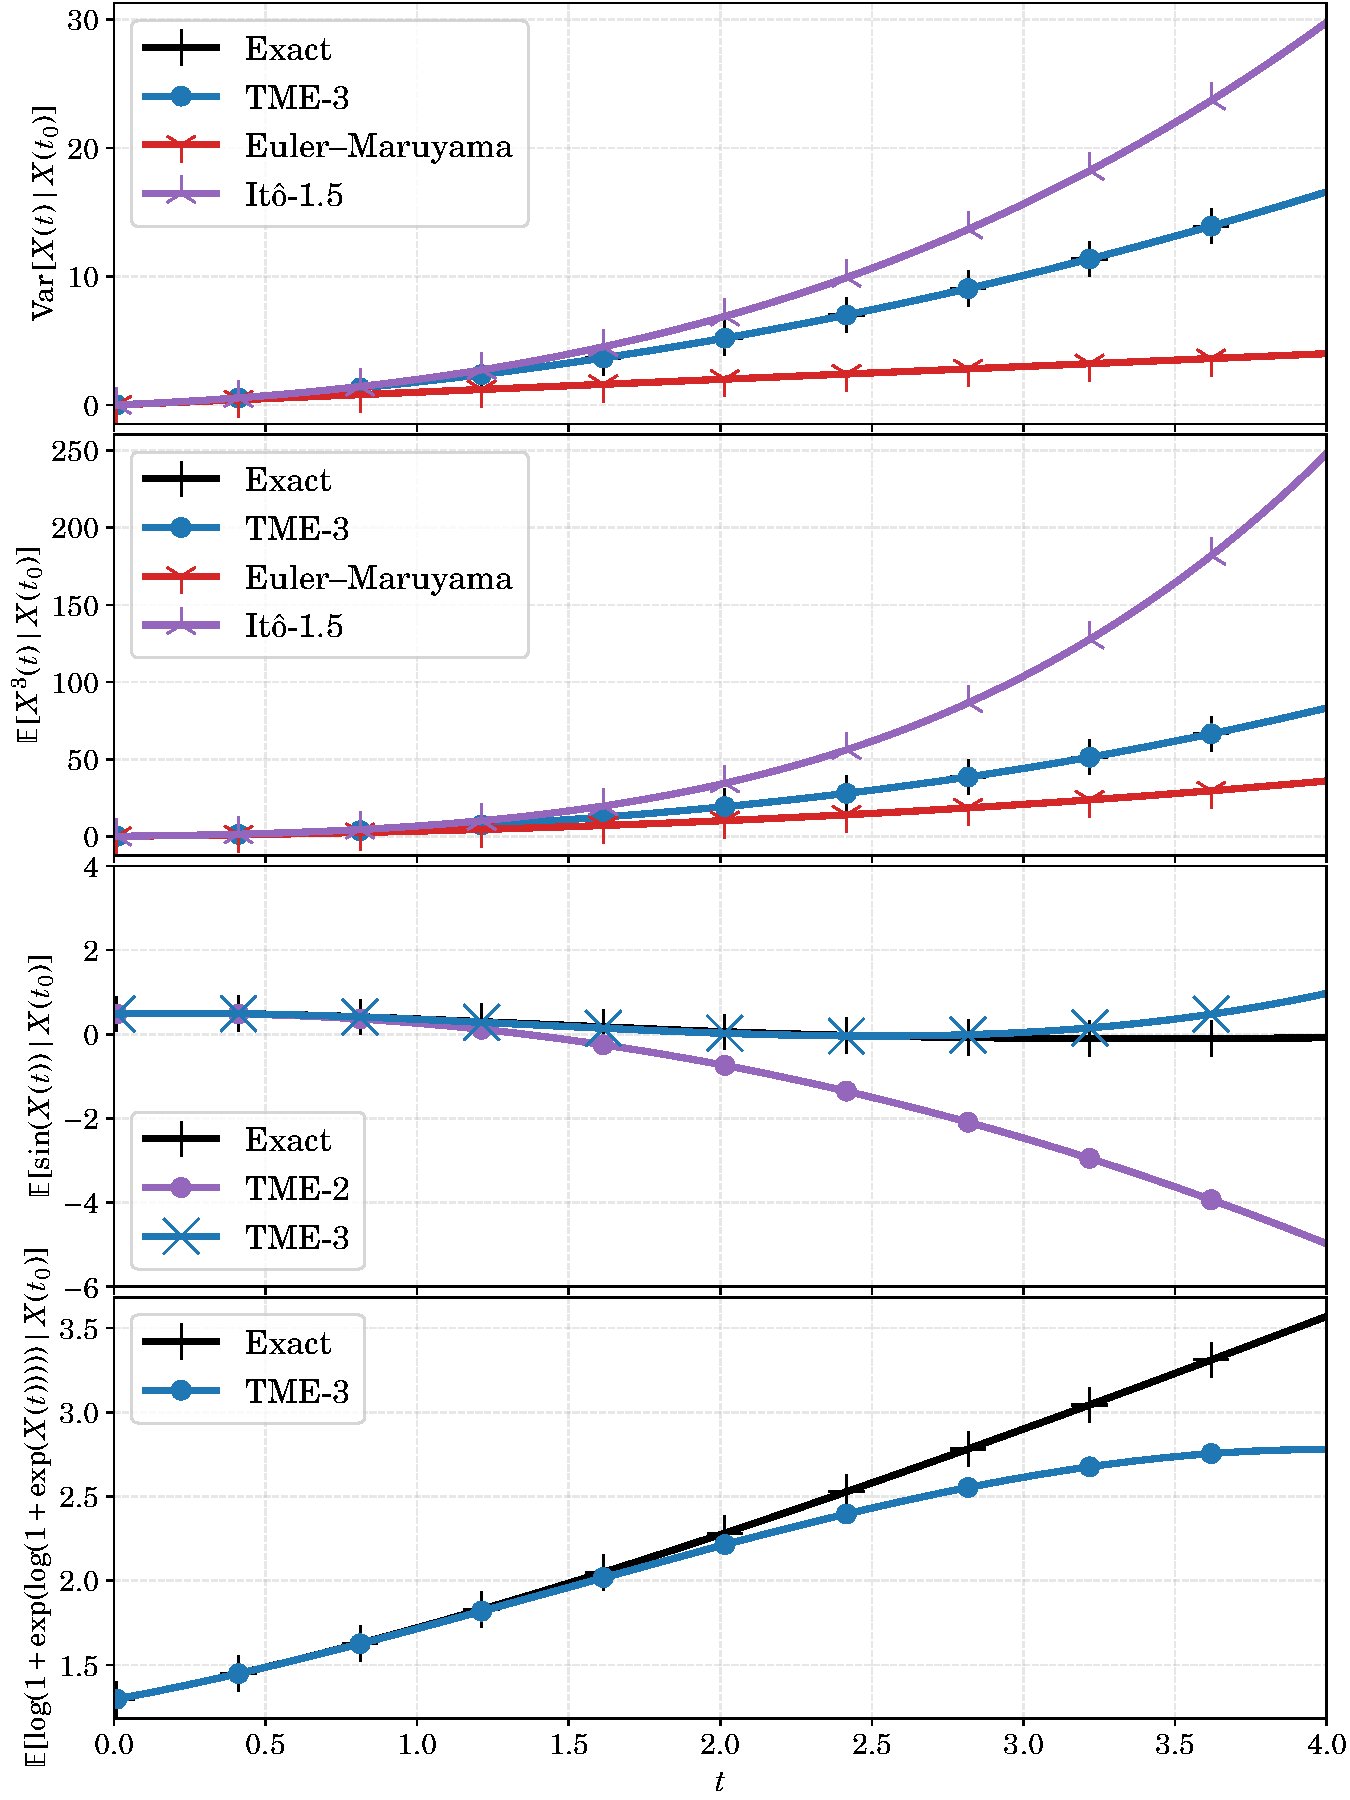
\includegraphics[width=.9\linewidth]{figs/tme-benes-all}
	\caption{Expectation approximations in Example~\ref{example-tme-benes}. The exact solutions are computed by numerical integration, as the transition density of the Bene\v{s} model is explicitly known~\citep[][Equation 10.58]{Sarkka2019}.}
	\label{fig:tme-benes}
\end{figure}

\begin{example}
	\label{example-tme-benes}
	Consider an It\^{o} process $X\colon \T \to \R$ which solves the Bene\v{s} model
	\begin{equation}
		\diff X(t) = \tanh(X(t)) \diff t + \diff W(t),
	\end{equation}
	starting from $X(t_0) = 0.5$. We are interested in computing its variance $\varr{X(t) \cond X(t_0)}$, third moment $\expec{X(t)^3 \cond X(t_0)}$, and two expectations 
	\begin{equation}
		\begin{split}
			&\expec{\sin(X(t)) \cond X(t_0)}, \\
			&\expec{\log(1+\exp(\log(1+\exp(X(t))))) \cond X(t_0)}.
		\end{split}
		\label{equ:tme-benes-nn}
	\end{equation}
	Notice that one can understand the last expectation above as a way to describe the propogation of $X$ through a neural network consiting of two single-neuron layers with Softplus activation functions.
	
	The TME-2 approximation for the variance $\varr{X(t) \cond X(t_0)}$ is exact. Specifically, $\Sigma_2(\Delta t) = \Delta t + (1-\tanh(X(t_0))^2)\,\Delta t^2$ is equal to $\varr{X(t) \cond X(t_0)}$.
\end{example}

In Figure~\ref{fig:tme-benes}, we plot the results for the expectations in Example~\ref{example-tme-benes}. In addition, we compare the TME method against the Euler--Maruyama and It\^{o}-1.5 methods. From the figure, we see that the TME approach outperforms the Euler--Maruyama and It\^{o}-1.5 methods significantly. Also, the TME approach can approximate the expectations in Equation~\eqref{equ:tme-benes-nn} to a good extent within a small time span.  Note that the Euler--Maruyama and It\^{o}-1.5 schemes do not give closed-form approximations for the expectations in Equation~\eqref{equ:tme-benes-nn}, we thus omit the two methods for these expectations. 

In the next example, we show how to use Theorem~\ref{thm:tme-cov-pd} and Corollary~\ref{corol-tme-pd-all-dt} in practice to analyse the positive definiteness of the TME covariance approximation of a non-linear multidimensional SDE. 

\begin{figure}[t!]
	\centering
	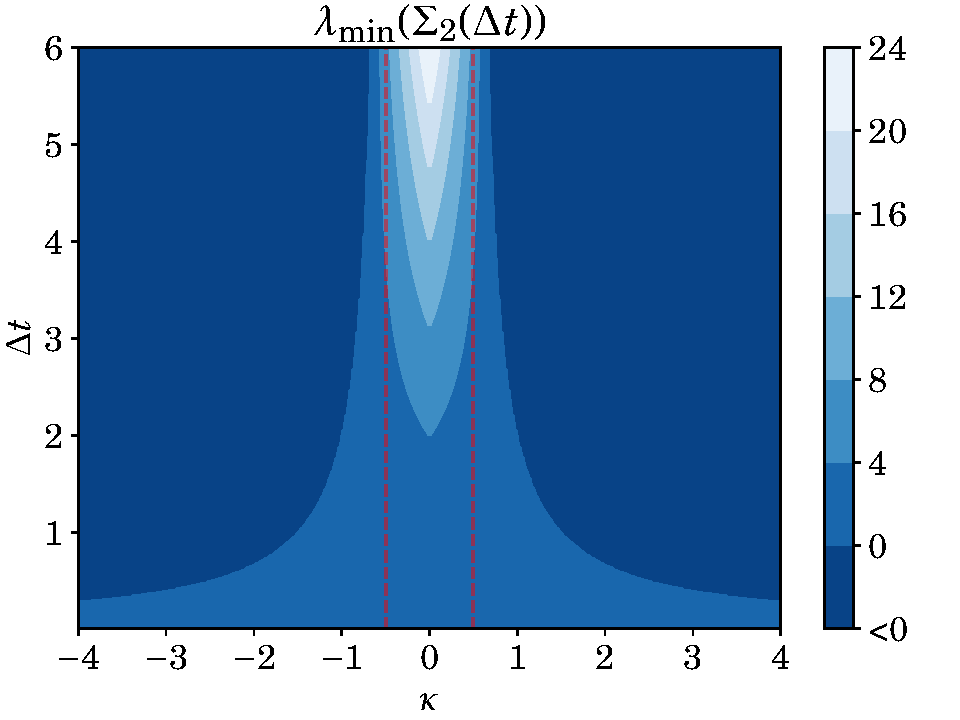
\includegraphics[width=.7\linewidth]{figs/tme-softplus-mineigs}
	\caption{Contour plot of the minimum eigenvalue of $\Sigma_2$ with respect to $\Delta t$ and $\kappa$ in Example~\ref{example:tme-softplus}. Red dashed lines stand for $\kappa=-0.5$ and $0.5$.}
	\label{fig:tme-softplus}
\end{figure}

\begin{example}
	\label{example:tme-softplus}
	Consider a two-dimensional SDE
	\begin{equation}
		\begin{split}
			\diff X^1(t) &= \bigl(\log(1 + \exp(X^1(t))) + \kappa \, X^2(t)\bigr) \diff t + \diff W_1(t), \\
			\diff X^2(t) &= \bigl(\log(1 + \exp(X^2(t))) + \kappa \, X^1(t)\bigr) \diff t + \diff W_2(t), 
		\end{split}
	\end{equation}
	where $\kappa \in \R$ is a tunable parameter. We want to ensure the positive definiteness of $\Sigma_2(\Delta t)$ for all $\Delta t \in \R_{>0}$ by tuning $\kappa$. In order to do so, we can first explicitly derive $\Theta_1$ and $\Theta_2$. It turns out that $\Theta_1$ is an identity matrix and
	\begin{equation}
		\Theta_2 = 2\,
		\begin{bmatrix}
			\frac{\expp^{X^1(t_0)}}{\expp^{X^1(t_0)}+1} & \kappa \\
			\kappa & \frac{\expp^{X^2(t_0)}}{\expp^{X^2(t_0)}+1}
		\end{bmatrix}.
	\end{equation}
	Then, by Corollary~\ref{corol-tme-pd-all-dt} it is sufficient to guarantee the positive definiteness of $\Sigma_2(\Delta t)$ for all $\Delta t\in\R_{>0}$ by ensuring that $\Theta_2$ is positive semi-definite. Thus, one should let 
	\begin{equation}
		\abs{\kappa} \leq \sqrt{\frac{\expp^{X^1(t_0) + X^2(t_0)}}{(\expp^{X^1(t_0)}+1) \, (\expp^{X^2(t_0)}+1)}} \nonumber.
	\end{equation}
	Figure~\ref{fig:tme-softplus} plots the minimum eigenvalues of $\Sigma_2(\Delta t)$ with respect to $\Delta t$ and $\kappa$ when $X^1(t_0)=X^2(t_0)=0$. In this case, $\abs{\kappa}$ should be less than $0.5$ (red dashed lines in the figure) in order to guarantee the positive definiteness of $\Sigma_2(\Delta t)$. The figure shows that $\Sigma_2(\Delta t)$ is indeed positive definite for all $\Delta t\in\R_{>0}$ within the region $\abs{\kappa}\leq 0.5$, and that this sufficient region is very close to the true region (i.e., the region of $\kappa$ that $\lambda_\mathrm{min}(\Sigma_2(\Delta t))>0$ for all $\Delta t$).
\end{example}

The positive definiteness analysis via Theorem~\ref{thm:tme-cov-pd} might be limited to simple SDEs and low orders of expansion. For $M\leq 3$, some explicit results can be stated as shown in Corollary~\ref{corol-tme-pd-all-dt}, but higher-order expansions can result in complicated polynomials to be analysed. 

\section{TME Gaussian filter and smoother}
\label{sec:tme-filter-smoother}

In the pioneering works by~\citet{Zmirou1986, Kessler1997, Sahalia2003}, the TME method was originally introduced for estimating unknown parameters of SDEs. More specifically, they use TME to discretise SDEs in order to perform maximum likelihood estimations. In this section, we show that the TME method could also be applied for solving Gaussian filtering and smoothing problems~\citep{ZhaoTME2020, ZhaoZTMEsmoother2021}.

Consider a (time-homogeneous) continuous-discrete state-space model
\begin{equation}
	\begin{split}
		\diff X(t) &= a(X(t)) \diff t + b(X(t)) \diff W(t), \quad X(t_0) = X_0,\\
		Y_k &= h(X_k) + \xi_k, \quad \xi_k \sim \mathrm{N}(0, \Xi_k),
	\end{split}
	\label{equ:tme-cd-model}
\end{equation}
where the solution $X\colon \T\to\R^d$ is observed through a non-linear function $h\colon \R^d\to\R^{d_y}$ and additive Gaussian noises $\lbrace \xi_k\colon k=1,2,\ldots \rbrace$. Furthermore, we assume that the SDE coefficients satisfy the conditions in Theorem~\ref{thm:tme}, so that we can apply the TME method. 

As shown in Algorithm~\ref{alg:gfs}, a key procedure of Gaussian filtering is to propagate the previous filtering result through the SDE and compute the predictive mean $m^-_k$ and covariance $P^-_k$. As for the Gaussian smoothing steps, one needs to compute the cross-covariance $D^-_{k+1}$ in Algorithm~\ref{alg:gfs}. These quantities can be approximated by using the TME method as follows.

Let us denote by $f^M$ and $Q^M$ the $M$-order TME approximations to the conditional mean and covariance (see, Lemma~\ref{lemma:tme-1-2-moments} and Theorem~\ref{thm:tme-cov-pd}), that are,
%
\begin{equation}
	\begin{split}
		\expec{X_k \cond X_{k-1}} &\approx f^M(X_{k-1}), \\
		\cov{X_k \cond X_{k-1}} &\approx Q^M(X_{k-1}).
	\end{split}
\end{equation}
%
Then by substituting $f^M$ and $Q^M$ into the prediction step in Algorithm~\ref{alg:gfs} we obtain the TME-approximated predictive mean and covariance
%
\begin{equation}
	\begin{split}
		&\int x_k \, p_{X_k \cond Y_{1:k-1}}(x_k \cond y_{1:k-1}) \diff x_k \\
		&= \iint x_k \, p_{X_k \cond X_{k-1}}(x_k \cond x_{k-1}) \, p_{X_{k-1} \cond Y_{k-1}} (x_{k-1} \cond y_{k-1}) \diff x_{k-1} \diff x_k\\
		&\approx \int f^M(x_{k-1}) \, \mathrm{N} \big(x_{k-1} \cond m^f_{k-1}, P^f_{k-1} \big) \diff x_{k-1}\\
		&= m^-_k, \\
		&\int (x_k - m_k^-) \, (x_k - m_k^-)^\trans \, p_{X_k \cond Y_{1:k-1}}(x_k \cond y_{1:k-1}) \diff x_k \\
		&\approx \int \Big(Q^M(x_{k-1}) + f^M(x_{k-1}) \, \big(f^M(x_{k-1})\big)^\trans \Big) \,\mathrm{N} \big(x_{k-1} \cond m^f_{k-1}, P^f_{k-1} \big) \diff x_{k-1} \\
		&\quad- m_k^- \, (m_k^-)^\trans \\
		&= P^-_k.
	\end{split}
	\label{equ:tme-gfs-pred}
\end{equation}
%
Similarly, for the cross-covariance $D_{k+1}$ in the smoothing pass we have
%
\begin{equation}
	\begin{split}
		&\iint x_k \, x_{k+1}^\trans \, p_{X_{k+1} \cond X_{k}}(x_{k+1} \cond x_{k}) \, p_{X_k \cond Y_{1:k}}(x_k \cond y_{1:k}) \diff x_k \diff x_{k+1} - m_k^f \, (m^-_{k+1})^\trans \\
		&\approx \int x_k \, \big(f^M(x_k)\big)^\trans \, \mathrm{N} \big(x_{k} \cond m^f_{k}, P^f_{k} \big)  \diff x_k  - m_k^f \, (m^-_{k+1})^\trans \\
		&= D_{k+1}.
	\end{split}
	\label{equ:tme-gfs-D}
\end{equation}
%
We formally define the TME Gaussian filter and smoother in the following algorithm.

\begin{algorithm}[TME Gaussian filter and smoother]
	\label{alg:tme-gfs}
	The algorithm is the same as Algorithm~\ref{alg:gfs}, except that the computations for the prediction (i.e., $m^-_k$ and $P^-_k$) and cross-covariance (i.e., $D_{k+1}$) are replaced by Equations~\eqref{equ:tme-gfs-pred} and~\eqref{equ:tme-gfs-D}, respectively.
\end{algorithm}

The expectations in Equations~\eqref{equ:tme-gfs-pred} and~\eqref{equ:tme-gfs-D} are usually computed by quadrature integration methods (e.g., sigma-point methods), since the approximations $f^M$ and $Q^M$ are usually non-linear functions. 

\subsection{Filter stability}
\label{sec:tme-stability}
The filter stability in this context refers to the error bound of the filtering estimates in the mean-square sense. For Kalman filters, some classical stability results are already shown, for example, by~\citet{Jazwinski1970} and~\citet{Anderson1981}. As for non-linear filters, their stability analyse has also been studied extensively in recent decades. For example, \citet{Reif1999} analyse the stability of extended Kalman filters, while the stability of more general Gaussian filters are found in~\citet{Kazufumi2000, Xiong2006}. There are also stability analysis that are model-specific. For instance, \citet{Blomker2013} and~\citet{LawK2014} analyse the stability of a class of Gaussian filters on the Navier--Stokes equation and a Lorenz model, respectively. In the remainder of this section, we rely on the stability results in~\citet{Toni2020} which apply for a wide class of non-linear filters and non-linear state-space models including ours. 

In this section, we analyse the stability of the TME Gaussian filters (see, Algorithm~\ref{alg:tme-gfs}) that use sigma-point integration methods for computing the expectations in Equation~\eqref{equ:tme-gfs-pred}. This analysis is necessary, as it is important to know if the TME Gaussian filtering error -- which accumulates in time -- is in some sense bounded. The sources of the error include, for example, TME approximations, Gaussian approximations to the filtering posterior distributions, and numerical integration. 

To proceed, let
%
\begin{equation}
	X_k = \check{f}(X_{k-1}) + \check{q}(X_{k-1})
\end{equation}
%
stand for the \textit{exact} discretisation of the SDE in Equation~\eqref{equ:tme-cd-model} for $k=1,2,\ldots$, where $\check{f}(X_{k-1}) \coloneqq \expec{X_k \cond X_{k-1}}$, and $\check{q}(X_{k-1})$ is a zero-mean random variable whose conditional covariance is $\check{Q}(X_{k-1}) \coloneqq \cov{\check{q}(X_k) \cond X_{k-1}}$. The principle of TME Gaussian filters is such that the TME method approximates $X_k$ via the discretisation
%
\begin{equation}
	X_k \approx f^M(X_{k-1}) + q^M(X_{k-1}),
\end{equation}
%
where $q^M(X_{k-1}) \sim \mathrm{N}(0, Q^M(X_{k-1}))$. By Theorem~\ref{thm:tme} or Lemma~\ref{lemma:tme-1-2-moments} we have 
%
\begin{equation}
	\check{f}(X_{k-1}) = f^M(X_{k-1}) + R_{M}(X_{k-1}),
\end{equation}
%
where we abbreviate the remainder by $R_{M}(X_{k-1}) \coloneqq R_{M, \phi^{\mathrm{I}}}(X_{k-1}, \Delta t_k)$.

Now suppose that we perform TME Gaussian filtering on a linearly-observed state-space model
%
\begin{equation}
	\begin{split}
		X_k &= \check{f}(X_{k-1}) + \check{q}(X_{k-1}),\\
		Y_k &= H \, X_k + \xi_k, \quad \xi_k\sim \mathrm{N}(0, R),
	\end{split}
	\label{equ:tme-stability-model}
\end{equation}
%
defined on a probability space $(\Omega, \FF, \PP)$, where $H \in \R^{d_y \times d}$ and $R\in\R^{d_y\times d_y}$ are constant matrices. Here, we limited ourselves to linear measurement models in order to use the preceding results by~\citet{Toni2020}. 

In the following, sigma-point approximations of Gaussian integrals of the form $\int z(x) \, \mathrm{N}(x \cond m, P) \diff x$ are denoted by $\mathcal{S}_{m, P}(z)$. The sigma-point TME Gaussian filter is such that the predictive mean in Algorithm~\ref{alg:tme-gfs} becomes $m^-_k = \mathcal{S}_{m^f_{k-1}, P^f_{k-1}}(f^M)$. 
\begin{remark}
	Sigma-point approximations of the form $\mathcal{S}_{m, P}(z)$ are weighted summations of $z$ evaluated at integration nodes that are determined by $m$, $P$, and their quadrature rules. For details of these, see, for example, \citet{Sarkka2013}.
\end{remark}

We show the stability of sigma-point TME Gaussian filters in the sense that 
%
\begin{equation}
	\sup_{k\geq 1}  \expecbigg{\normbig{X_k - m^f_k}^2_2} < \infty.
	\label{equ:tme-stability-aim}
\end{equation}
%
\begin{remark}
	Note that if $m^f_k = \expec{X_k \cond Y_{1:k}}$ is obtained exactly, then the mean-square in the equation above is minimised, since $\expec{X_k \cond Y_{1:k}}$ is an orthogonal projection of $X_k$. But in practice, one can only hope for approximating $\expec{X_k \cond Y_{1:k}}$ by using, for example, TME Gaussian filters. The stability analysis here is devoted to show that the TME Gaussian filtering error has a finite (contractive) bound that depends on step $k$.
\end{remark}

We use the following assumptions.

\begin{assumption}
	\label{assump:tme-stability-sys}
	There exist constants $c_M \geq 0$, $c_{\check{q}} \geq 0$, and $c_P \geq 0$ such that $\sup_{k\geq 1} \norm{R_M(X_{k-1})}_2 \leq c_M$ $\PP$-almost surely, $\sup_{k\geq 1} \expecbig{\tracebig{\check{Q}(X_{k-1})}} \leq c_{\check{q}}$, and $\sup_{k\geq 1} \expecbig{\trace{P^f_k}} \leq c_P$.
\end{assumption}

\begin{assumption}
	\label{assump:tme-stability-sp}
	There exists $c_\mathcal{S}\geq 0$ such that
	%
	\begin{equation}
		\normbig{f^M(x) - \mathcal{S}_{m, p}(f^M)}^2_2 \leq \normbig{ \jacob_x f^M(x) }^2_2 \, \norm{x - m}^2_2 + c_\mathcal{S} \trace{P},
	\end{equation}
%
	for all $x \in \R^d$, $m \in \R^d$, and positive semi-definite matrix $P \in \R^{d\times d}$.
\end{assumption}

\begin{assumption}
	\label{assump:tme-stability-k}
	There exists $c_K \geq 0$ such that $\sup_{k \geq 1} \norm{I - K_k \, H}_2 \leq c_K$ $\PP$-almost surely, and
	%
	\begin{equation}
		c_f^2 \coloneqq c_K^2 \, \sup_{x \in \R^d} \! \normbig{\jacob_x f^M(x)}_2^2 < \frac{1}{4}.
	\end{equation}
	%
\end{assumption}
Indeed, the assumptions above are in some sense restrictive. In particular, the TME remainder and the covariance of the transition density are required to be bounded by $c_M$ and $c_{\check{q}}$, respectively. In order to satisfy these assumptions, it is sufficient to require that the SDE coefficients are smooth enough and all their derivatives up to a certain order are uniformly bounded (e.g., the Bene\v{s} model in Example~\ref{example-tme-benes}). For more detailed explanations of these assumptions can be found in~\citet{ZhaoTME2020} and~\citet{Toni2020}.

The main result is shown in the following theorem.

\begin{theorem}[TME Gaussian filter stability]
	\label{thm:tme-stability}
	Suppose that Assumptions~\ref{assump:tme-stability-sys} to~\ref{assump:tme-stability-k} hold. Then the sigma-point TME Gaussian filter for system~\eqref{equ:tme-stability-model} is such that 
	%
	\begin{equation}
		\begin{split}
			\expecbigg{\normbig{X_k - m^f_k}^2_2} &\leq \big(4\, c_f^2\big)^k \trace{P_0}  \\
			&\quad+ \frac{4 \, \big( c_K^2 \,\big(c_\mathcal{S} \, c_P + c_M^2 + c_{\check{q}}\big) + \trace{R}  \, c_P^2 \, \norm{H}_2^2 \, \norm{R^{-1}}^2_2 \big)}{1 - 4\, c_f^2}.
		\end{split}
		\label{equ:tme-stab-bound}
	\end{equation}
	%
\end{theorem}
\begin{proof}
	Define $Z_k \coloneqq I - K_k \, H$. By substituting the sigma-point TME Gaussian filtering steps and the model~\eqref{equ:tme-stability-model} in $X_k - m^f_k$, we get
	%
	\begin{equation}
		\begin{split}
			X_k - m^f_k &= \check{f}(X_{k-1}) + \check{q}(X_{k-1}) - m^-_k - K_k \, (Y_k - H \, m^-_k), \\
			&= Z_k \, \Big( \check{f}(X_{k-1}) - \mathcal{S}_{m^f_{k-1}, P^f_{k-1}}(f^M) + \check{q}(X_{k-1}) \Big) - K_k \, \xi_k \\
			&= Z_k \, \Big( f^M(X_{k-1}) - \mathcal{S}_{m^f_{k-1}, P^f_{k-1}}(f^M)\Big) \\
			&\quad+Z_k \, R_{M}(X_{k-1}) + Z_k \, \check{q}(X_{k-1}) - K_k \, \xi_k.
		\end{split}
	\end{equation}
	%
	Then 
	%
	\begin{align}
		\expecbigg{\normbig{X_k - m^f_k}_2^2} &\leq 4 \, \expecBigg{ \normBig{Z_k \, \Big( f^M(X_{k-1}) - \mathcal{S}_{m^f_{k-1}, P^f_{k-1}}(f^M)\Big)}^2_2 } \label{equ:tme-stab-e}\\
		&\quad+ 4 \, \Big( \expecbig{\norm{Z_k \, R_{M}(X_{k-1})}^2_2} + \expecbig{\norm{Z_k \, \check{q}(X_{k-1})}^2_2} + \expecbig{\norm{K_k \, \xi_k}_2^2} \Big). \nonumber
	\end{align}
	%
	Now, by substituting the bounds 
	%
	\begin{equation}
		\begin{split}
			\expecBigg{ \normBig{Z_k \, \Big( f^M(X_{k-1}) - \mathcal{S}_{m^f_{k-1}, P^f_{k-1}}(f^M)\Big)}^2_2 } &\leq c_f^2 \, \expecbigg{\normbig{X_{k-1} - m^f_{k-1}}_2^2} \\
			&\quad+ c_K^2 \, c_\mathcal{S} \, c_P, \\
			\expecbig{\norm{Z_k \, R_{M}(X_{k-1})}^2_2} &\leq c_K^2 \, c_M^2, \\
			\expecbig{\norm{Z_k \, \check{q}(X_{k-1})}^2_2} &\leq c_K^2 \, c_{\check{q}}, \\
			\expecbig{\norm{K_k \, \xi_k}_2^2} &\leq \trace{R}  \, c_P^2 \, \norm{H}_2^2 \, \norm{R^{-1}}^2_2,
		\end{split}
	\end{equation}
	%
	following Assumptions~\ref{assump:tme-stability-sys},~\ref{assump:tme-stability-sp}, and~\ref{assump:tme-stability-k} into Equation~\eqref{equ:tme-stab-e}, we obtain the recursive inequality
	%
	\begin{equation}
		\begin{split}
			\expecbigg{\normbig{X_k - m^f_k}_2^2} &\leq 4 \, c_f^2 \, \expecbigg{\normbig{X_{k-1} - m^f_{k-1}}_2^2} \\
			&\quad+ 4 \, \big( c_K^2 \,\big(c_\mathcal{S} \, c_P + c_M^2 + c_{\check{q}}\big) + \trace{R}  \, c_P^2 \, \norm{H}_2^2 \, \norm{R^{-1}}^2_2 \big).
		\end{split}
	\end{equation}
	%
	The assumption $4 \, c_f^2< 1$ concludes the bound in Equation~\eqref{equ:tme-stab-bound}.
\end{proof}

Stability analysis of Gaussian smoothers that use the TME method can be found in~\citet{ZhaoZTMEsmoother2021}.

\subsection{Signal estimation and target tracking examples}
\label{sec:tme-gfs-examples}
This section presents a few applications of TME Gaussian filters and smoothers on signal estimation and target tracking problems. In the examples below, we uniformly use the expansion order $M=3$, and we use the Gauss--Hermite quadrature method (of order 3) to approximate the Gaussian expectations in Equations~\eqref{equ:tme-gfs-pred} and~\eqref{equ:tme-gfs-D}.

\begin{example}[Bene\v{s}]
	\label{example:tme-benes-filter-smoother}
	Consider the Bene\v{s} model in Example~\ref{example-tme-benes}, and also consider a linear measurement model $Y_k = X(t_k) + \xi_k$, where $\xi_k \sim \mathrm{N}(0, 0.5)$. We simulate a pair of a signal and its measurements at times $\lbrace t_k=0.01 \, k \colon k=0,1,\ldots, 500 \rbrace$, then we apply the TME-3 Gaussian filter and smoother to estimate the signal from the measurements. The results are plotted in Figure~\ref{fig:tme-benes-filter-smoother}.
\end{example}

\begin{figure}[t!]
	\centering
	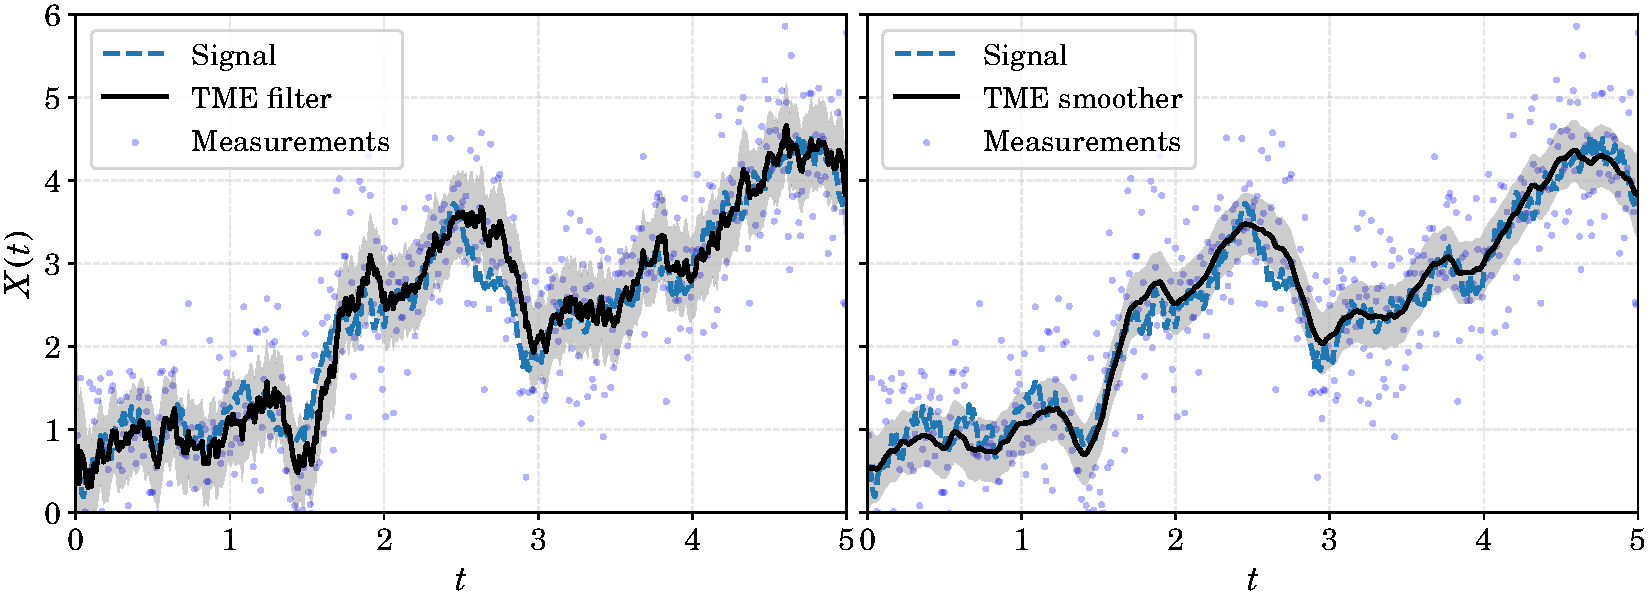
\includegraphics[width=.99\linewidth]{figs/tme-benes-filter-smoother}
	\caption{TME Gaussian filtering and smoothing for the Bene\v{s} model in Example~\ref{example:tme-benes-filter-smoother}. Shaded area stands for $0.95$ confidence interval.}
	\label{fig:tme-benes-filter-smoother}
\end{figure}

\begin{figure}[t!]
	\centering
	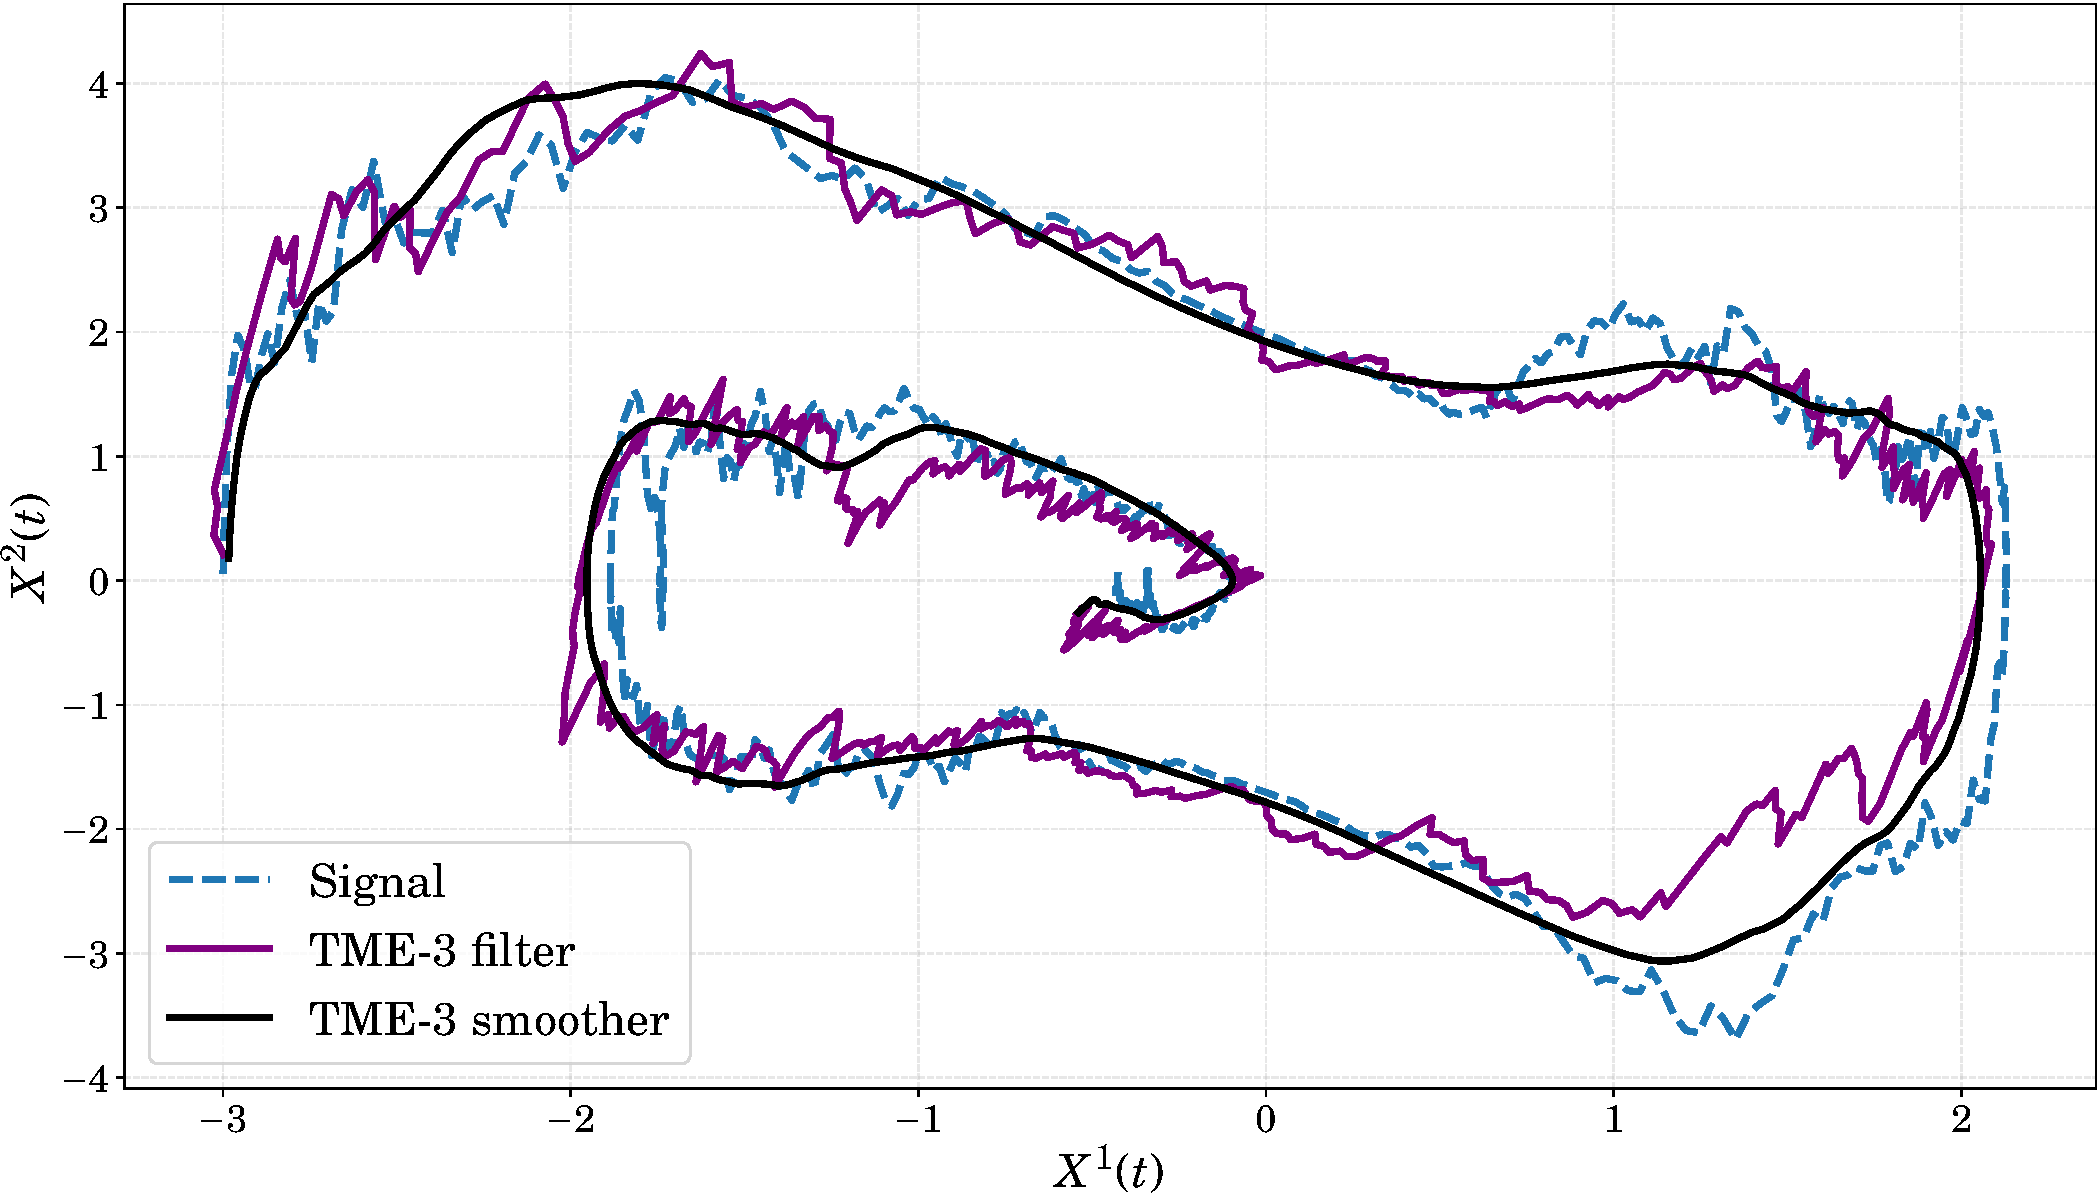
\includegraphics[width=.9\linewidth]{figs/tme-duffing-filter-smoother} \\
	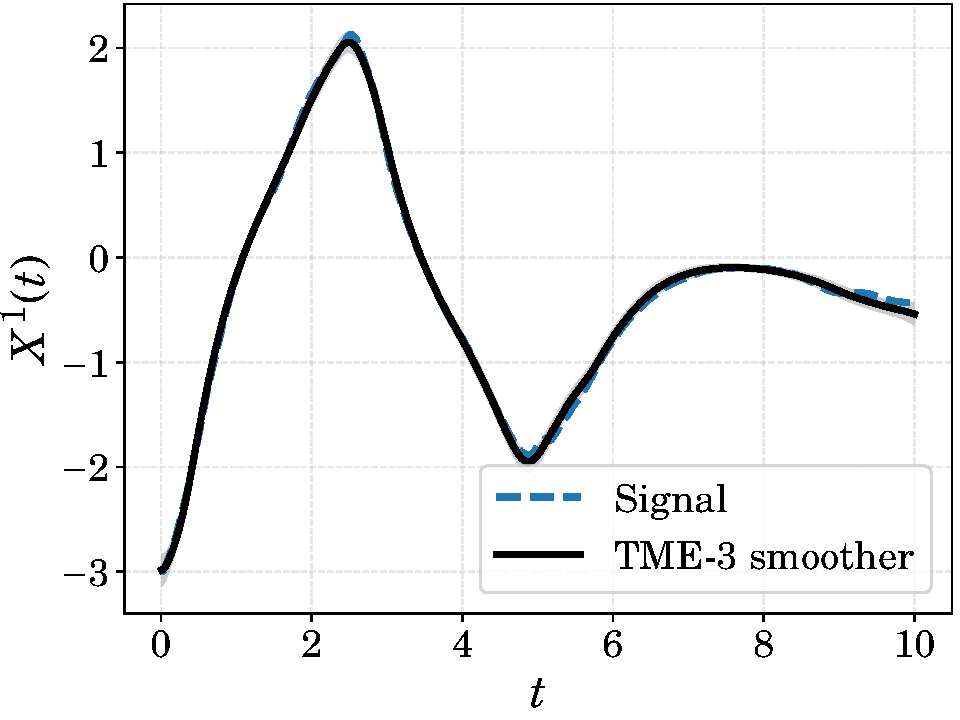
\includegraphics[width=.494\linewidth]{figs/tme-duffing-smoother-x1}
	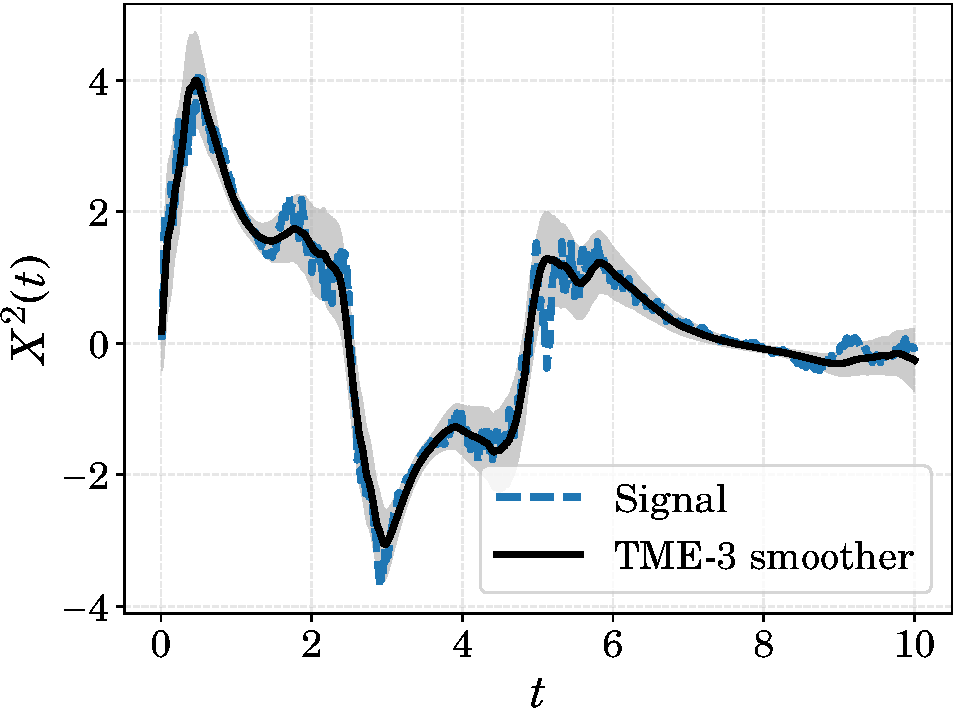
\includegraphics[width=.494\linewidth]{figs/tme-duffing-smoother-x2}
	\caption{TME Gaussian filtering and smoothing for the Duffing--van der Pol model in Example~\ref{example:tme-duffing-filter-smoother}. }
	\label{fig:tme-duffing-filter-smoother}
\end{figure}

\begin{example}[Duffing--van der Pol]
	\label{example:tme-duffing-filter-smoother}
	Consider a continuous-discrete state-space model
	%
	\begin{equation}
	\begin{split}
	\diff X^1(t) &= X^2(t) \diff t, \\
	\diff X^2(t) &= \Big(X^1(t) \, \big(\kappa - \big(X^1(t)\big)^2\big) - X^2(t) \Big) \diff t + X^1(t) \diff W(t), \\
	Y_k &= X^1(t_k) + 0.1 \, X^2(t_k) + \xi_k,
	\end{split}
	\end{equation}
	%
	starting from the initial values $X^1(t_0) = -3$ and $X^2(t_0)=0$, where $\kappa = 2$ and $\xi_k \sim \mathrm{N}(0, 0.1)$. The non-linear multiplicative SDE above is called a modified stochastic Duffing--van der Pol oscillator equation~\citep{Lord_powell_shardlow_2014, Sarkka2019}. We simulate a pair of a signal and its measurements at times $\lbrace t_k=0.01\,k \colon k=0,1,\ldots,1000 \rbrace$. The results of the TME-3 Gaussian filtering and smoothing for this model is illustrated in Figure~\ref{fig:tme-duffing-filter-smoother}. 
	
	It is worth mentioning that the Euler--Maruyama-based Gaussian smoothing methods on this model may encounter numerical problems because the Euler--Maruyama scheme gives singular covariance approximation.
\end{example}

\begin{figure}[t!]
	\centering
	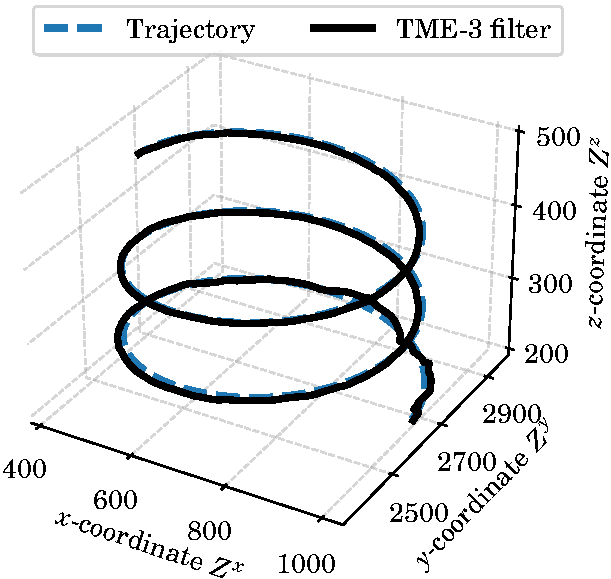
\includegraphics[width=.494\linewidth]{figs/tme-ct3d-filter}
	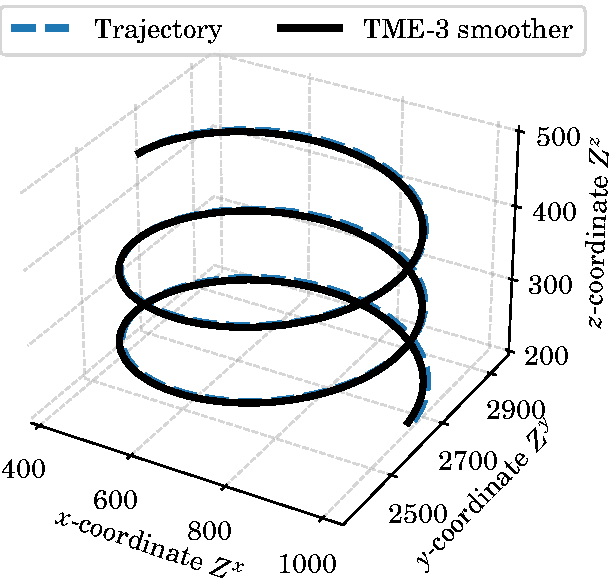
\includegraphics[width=.494\linewidth]{figs/tme-ct3d-smoother}
	\caption{TME Gaussian filtering and smoothing for tracking a target moving as per the 3D coordinated turn model in Example~\ref{example:tme-ct-tracking}. }
	\label{fig:tme-ct3d}
\end{figure}

\begin{example}[3D coordinated turn tracking]
	\label{example:tme-ct-tracking}
	Consider a continuous-discrete model
	%
	\begin{equation}
		\begin{split}
			\diff Z(t) &= a^{\mathrm{CT}}(Z(t)) \diff t + b^{\mathrm{CT}} \diff W(t), \\
			Y_k &= h^{\mathrm{CT}}(Z(t_k)) + \xi_k,
		\end{split}
	\end{equation}
	%
	where the state $Z \colon \T \to \R^7 \coloneqq \begin{bmatrix} Z^x(t) & \dot{Z}^x(t) & Z^y(t) & \dot{Z}^y(t) & Z^z(t) & \dot{Z}^z(t) & \vartheta(t)\end{bmatrix}^\trans$ stands for the 3D Cartesian coordinate and the turn rate of a target. The SDE coefficients and the measurement function are defined by
	%
	\begin{equation}
		\begin{split}
			a^{\mathrm{CT}}(Z(t)) &= 
			\begin{bmatrix}
				\dot{Z}^x(t) & - \vartheta(t) \, \dot{Z}^y(t) & \dot{Z}^y(t) & \vartheta(t) \, \dot{Z}^x(t) & \dot{Z}^x(t) & 0 & 0
			\end{bmatrix}^\trans, \\
			h^{\mathrm{CT}}(Z(t_k)) &= 
			\begin{bmatrix}
				\sqrt{(Z^x(t_k))^2 + (Z^y(t_k))^2 + (Z^z(t_k))^2} \\
				\arctan(Z^y(t_k) \, / \, Z^x(t_k)) \\
				\arctan\bigl(Z^z(t_k) \, / \, \sqrt{(Z^x(t_k))^2 + (Z^y(t_k))^2}\bigr)
			\end{bmatrix}.
		\end{split}
	\end{equation}
	%
	For details of this model, we refer the reader to~\citet{ZhaoTME2020}. This model is widely used for manoeuvring target tracking and is very challenging for filtering and smoothing algorithms due to its high dimensionality and non-linearity~\citep{CDCKF2010, BarShalom2002}. A tracking example by using the TME-3 Gaussian filter and smoother is shown in Figure~\ref{fig:tme-ct3d}.
\end{example}
